\chapter{test}

本章主要介绍仿真环境的搭建

\section{仿真环境搭建}

\begin{equation}
\begin{pmatrix} 
3 & 4 & 5 \\
0 & 1 & 2 \\
9 & 8 & 7  
\end{pmatrix}=
\begin{bmatrix} 
x_1 & x_2 & x_3 \\
y_1 & y_2 & y_3 \\
z_1 & z_2 & z_3 
\end{bmatrix} 
\end{equation}

\begin{lstlisting}[language={[ANSI]C}] 
int main(int argc, char ** argv) 
{ 
printf("Hello world! \n"); 
return 0; 
} 
\end{lstlisting}

\begin{algorithm}
\caption{A test algorithm (Part I)}
\begin{algorithmic}[1]
\Require <hahdsfasdfadf>
\Ensure <hahdsfasdfadf>
\State <hahdsfasdfadf>
\If{<condition>}
	\State <hahdsfasdfadf>
\ElsIf{<condition>}
	\State <hahdsfasdfadf>
\Else 
	\State <hahdsfasdfadf>
\EndIf
\For{<condition>}
	\State <hahdsfasdfadf>
\EndFor
\ForAll{<condition>}
	\State <hahdsfasdfadf>
\EndFor
\While{<condition>}
	\State <hahdsfasdfadf>
\EndWhile
\Repeat
	\State <hahdsfasdfadf>
\Until{<condition>}
\Loop
	\State <hahdsfasdfadf>
\EndLoop
    \algstore{bkbreak}
\end{algorithmic}
\end{algorithm}

\begin{algorithm}
\caption*{A test algorithm (Part II)}
\begin{algorithmic}[1]
\algrestore{bkbreak}
\Function{<name>}{<params>} <body> \EndFunction
\State \Return <hahdsfasdfadf>
\Comment{<comment>}
\Procedure {BellmanKalaba}{$G$, $u$, $l$, $p$}
\ForAll {$v \in V(G)$}
\State $l(v) \leftarrow \infty$
\EndFor
\State $p(i) \leftarrow v_j$
\State $l’(i) \leftarrow min$
\State $changed \leftarrow l \not= l’$
\EndProcedure
\end{algorithmic}
\end{algorithm}

% \begin{algorithm}[H]
% \caption{How to write algorithms}
% \KwIn{this text}
% \KwOut{how to write algorithm with \LaTeX2e }
% initialization\;
% \While{not at end of this document}{
%     read current\;
%     \eIf{understand}{
%         go to next section\;
%         current section becomes this one\;
%     }{
%         go back to the beginning of current section\;
%     }
% }
% \end{algorithm}

空行:
\newline

随机蕨最早由他[\citenum{ozuysal2007fast}]提出\cite{ozuysal2007fast}。

项目:\\
无序:
\begin{itemize}
\item[-] good morning...
\item[-] good morning....
\end{itemize}

\begin{itemize}
\item good evening...
\item good evening....
\end{itemize}

有序:
\begin{enumerate}
\item good morning...
\item good morning....
\end{enumerate}

公式:
\begin{equation}
	a^2=b^2+c^2+d^2
\end{equation}

行内公式:
balabala
$P(C_k|F)$
balabala

% Listing~\ref{lst:}

\begin{equation}
	OK
\end{equation}

图像:
\begin{figure}[htb]
	\centering 
	% 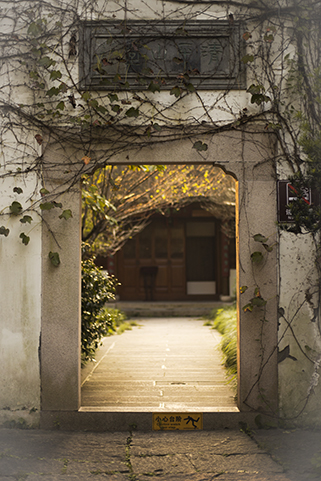
\includegraphics[width=\textwidth]{./Pictures/test.jpg} 
	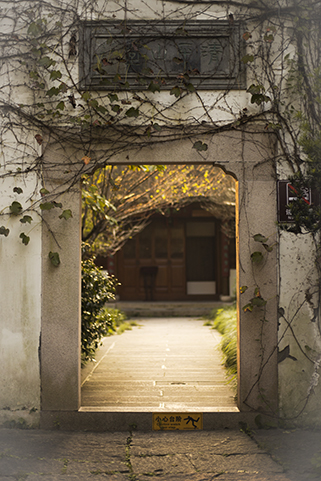
\includegraphics[scale=1.0]{./Pictures/test.jpg} 
	\caption{ljzst} 
\end{figure}

\begin{figure}[htb]
	\centering 
	% 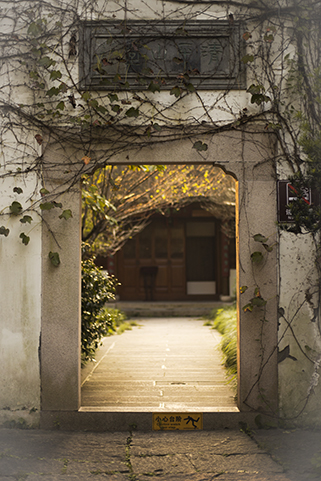
\includegraphics[width=\textwidth]{./Pictures/test.jpg} 
	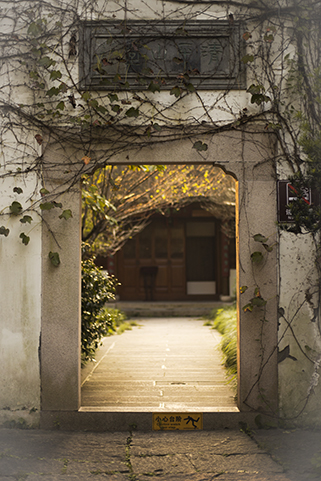
\includegraphics[scale=1.0]{./Pictures/test.jpg} 
	\caption{another way} 
\end{figure}

\begin{figure}[htb]
	\subfigure[img1]{ 
		\begin{minipage}[b]{0.5\textwidth} 
		\centering
		% \label{fig:SubFigure1} %% label for second subfigure 
		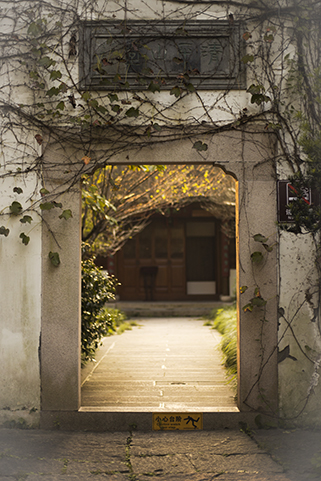
\includegraphics[scale=1.0]{./Pictures/test.jpg} 
		\end{minipage}}
	\subfigure[img2]{ 
		\begin{minipage}[b]{0.5\textwidth} 
		\centering
		% \label{fig:SubFigure1} %% label for second subfigure 
		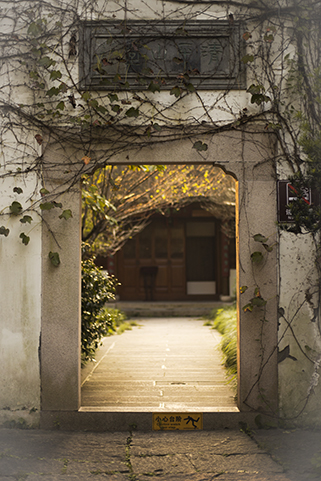
\includegraphics[scale=1.0]{./Pictures/test.jpg} 
		\end{minipage}}
	\caption{img all}
\end{figure}

{
\begin{table}[htb]
	\zihao{5}
	\caption{standard table} 
	% \label{Tabkeyword}
	\centering 
	\begin{tabular}[t]{
		|c|l|r|p{4cm}|} 
		\hline
		center & left & right & 靠左,并宽4cm\\ 
		\hline
		Center & Left & Right & Width=4cm\\ 
		\hline
	\end{tabular}
\end{table}
}

{
\begin{table}[htp]
	\zihao{5}
	\caption{复杂表格示例}
	% \label{TabComplex}
	\centering
	\begin{tabular}[t]{|c|c|c|c|c|}
		\hline
		\multicolumn{2}{|c|}{我占了两列} & 第3列 & 第4列 & 第5列\\
		\hline
		\multirow{2}*{我占了两行} & 第二行第2列 & 第二行第3列 & \multicolumn{2}{|c|}{\multirow{2}*{我占了两行又两列}}\\
		\cline{2-3}
		& 第三行第2列 & 第三行第3列 & \multicolumn{2}{|c|}{} \\
		\hline
	\end{tabular}
\end{table}
}



\section{OpenGL}

\subsection{投影变换}